\chapter{Experiments}
\label{chap:experiments}

\section{Experimental Project Data}
\label{sec:experimental_project_data}

One thing that should be noted for the experiments that were run. Since all of the data was known before the model was even created artificial cut off dates were created to allow for the feature set to be tested as to their effect on the model. A test project, acra (developed by the user ACRA), was chosen to develop the method on. 

%The project data was extracted from GitHub from when the project was initially committed to GitHub (2010-04-18 15:52:18-04) till the cut off day of extraction (2015-06-05 09:02:56-04). The cut off day was the day the data was extracted from GitHub and after of which the data analysis was initiated.

% TODO consider placing this into introduction
\begin{table}[h!]
\begin{minipage}{\textwidth}
\begin{center}
    \begin{tabular}{|c|c|c|c|c|c|}
        \hline
        Owner & Project & Start Date & End Date & \# of & \# of \\
         & & & & Commits & Developers \\
        \hline
        ACRA & acra\footnote{\url{https://github.com/ACRA/acra}} & 2010-04-18 & 2015-06-05 & 404 & 32 \\
        apache & storm\footnote{\url{https://github.com/apache/storm}} & 2011-09-16 & 2015-12-28 & 2445 & 261 \\
        facebook & fresco\footnote{\url{https://github.com/facebook/fresco}} & 2015-03-26 & 2015-10-30 & 313 & 47 \\
        square & dagger\footnote{\url{https://github.com/square/dagger}} & 2012-06-25 & 2016-01-30 & 496 & 39 \\
        deeplearning4j & deeplearning4j\footnote{\url{https://github.com/deeplearning4j/deeplearning4j}} & 2013-11-27 & 2016-02-13 & 3523 & 62 \\
        \hline
    \end{tabular}
\end{center}
\caption{Experiment projects}
\label{tab:project_summary}
\end{minipage}
\end{table}

The complete list of projects that were tested is found in \autoref{tab:project_summary}. The number of commits excludes any commit that lacked a change to a file containing Java code. Since the primary interest was to parse Java code, files containing Java code were used while all other files are ignored. These measures provide a more accurate description of the project in terms of the analysis and predictions made on it. Secondly, the number of developers does not map effectively to what git uses as committers and authors. Instead, the number of developers includes all individuals (removing duplicates) who committed or authored commits to the current project.

%TODO place the tables in better positions.
\begin{table}
\begin{center}
    \begin{tabular}{|c|c|c|c|c|c|}
        \hline
        Project & \# of Methods & \# of Methods & Avg \# of & Avg \# of Methods \\
         & & Changes & Commits / Year & Change / Commit \\
        \hline
        acra & 1309 & 3605 & 67.33 & 9.51 \\
        storm & 14599 & 50037 & 489 & 24.03 \\
        fresco & 3463 & 4139 & 313 & 14.73 \\
        dagger & 1827 & 6314 & 99.2 & 13.70 \\
        deeplearning4j & 29896 & 82198 & 880.75 & 24.33 \\
        \hline
    \end{tabular}
\end{center}
\caption{Project Change Statistics}
\label{tab:project_stats}
\end{table}

Each of the projects selected on GitHub using the list of Java projects with a large amount of contributions. Open source projects were targeted to simplify any usage concerns. Therefore in order to be selected the program had to clearly use an \gls{oss} license. Secondly, the program also needed to have at least a 6 months worth of development and at least 300 commits to provide a large enough dataset to analyze. An effort was also made to pick projects of different sizes to provide better tests of various conditions.

The first project acra is a Android bug logging tool used with Android applications to capture information related to bugs or crashes. The information is sent to the developers to help them address the issues that their clients encounter while using there application. The second project, apache's storm, real time computational system for continuous streams of data. This project is one of the larger projects and has a large development community. The third project, facebook's fresco, is the smallest project with the shortest development period. This project provides a library for using images on Android to attempt to solve limited memory issues with mobile devices. The fourth project, square's dagger, is a Java application used to satisfy dependencies for classes to replace the factory model of development. The final project, deeplearning4j, is a distributed neural network library that integrates Hadoop and Spark. This application is the largest of the 5 projects and provides a large wealth of data to analyze.

\begin{table}
\begin{center}
    \begin{tabular}{|c|c|c|c|c|c|}
        \hline
        Project & Avg \# of & Avg \# of & Avg \# of & Max & Min \\
         & Methods Change & Changes & Commits / & Commits & Commits \\
         & / Year & / Method & Developer & / Year & / Year \\
        \hline
        acra & 600.83 & 4.52 & 13.93 & 119 & 33 \\
        storm & 10007.4 & 5.93 & 15.47 & 948 & 118 \\
        fresco & 4139 & 1.49 & 156.5 & 313 & 313 \\
        dagger & 1578.5 & 5.64 & 16 & 236 & 4 \\
        deeplearning4j & 20549.5 & 5.69 & 65.24 & 2018 & 65 \\
        \hline
    \end{tabular}
\end{center}
\caption{Project Change Statistics 2}
\label{tab:project_stats_2}
\end{table}

In order to get a more detailed understand of the selected projects numerous measures were taken. These measures also allow for each projects to be compared to each other in terms of the development of each of the projects. The size of the project is represented through number of commits, methods. The size of the development team is also provided. The length of each project is shown and most of the measures average on a yearly term.

% TODO reference the table
Several average measures were also taken which detail the amount of change that occurs within the project. The average number of commits per project coupled with the average number of changes per commit clearly indicates the amount of changes that are occurring with in the project. The rate at which methods are change provides good insight into the growth of a project. While some changes may involve the addition of new methods, others may include the removal of methods or the modification of methods. The other measures relating to the amount of change occurring with a project on average are the number of methods changed per year and the number of changes per method. Each of these further outline how the changes are being made to the project on average.

A few of the measures are related to the number of developers. These while provided are not the primary focus. The information provided by tracking developer interactions with each other or the repository could be integrated into future work.

\begin{table}
\begin{center}
    \begin{tabular}{|c|c|c|c|c|c|c|}
        \hline
        Project & Max \# of & Min \# of & Max \# of & Min \# of & Max \# of & Min \# of \\
         & Methods & Methods & Change / & Change / & Commits / & Commits / \\
         & Changed & Changed & Method & Method & Developer & Developer \\
         & / Year & / Year & & & & \\
        \hline
        acra & 1503 & 183 & 52 & 1 & 229 & 1 \\
        storm & 26526 & 2152 & 314 & 1 & 622 & 1\\
        fresco & 4139 & 4139 & 33 & 1 & 269 & 44 \\
        dagger & 3374 & 171 & 65 & 1 & 157 & 1 \\
        deeplearning4j & 35869 & 4377 & 345 & 1 & 1987 & 1 \\
        \hline
    \end{tabular}
\end{center}
\caption{Project Change Statistics 3}
\label{tab:project_stats_3}
\end{table}

While the purposed method was being developed ACRA's acra project was primarily used for exploring and initial testing of the approach. After experimenting on acra a few of the potential candidate feature sets were distinguished based on their superior performance. Experiments were then run on other projects using the feature sets that performed better.

    % An effort was made to not count individuals twice however some users may have changed their user name and thus showed up several times.
% NOTE the number of commits is the number of commits that contained Java code and thus was useful towards parsing.
% Note the number of developers is the total number of developers who both committed or authored commits, aka people who made pull requests are included.

% TODO merge the different experiment notes sections into one subsection

% \subsection{Experiment 1}

% % TODO look for test results for this one
% The first set of experiments were preliminary and used \gls{svm} as the approach for prediction algorithm. They attempted to predict whether a given method would change within the next 6 commits. The test was done one using ACRA's acra (hence forth just called \textit{acra}). The data set was divided into four sections based on the date length. So each section of the data was the project's lifespan divided by 4 long. The sampling method from the data set $data_i$ was to use the first $n$ tuples ordered by date. The value of $n$ was tested at 100 and 1000. The data set $data_i$ contained tuples which had changes and ones that had no changes.

% $|data_i| = \frac{|date_f - date_s|}{4}$

% The results of these experiments were not particularly promising scoring accuracy, precision, recall and recall around $50\%$ or below. The experiment was run such that $data_i$ would be used for training and $data_{i+1}$ would be used for testing. For example $data_1$ would be used to train $model_{1,2}$ and $data_2$ would be used to test the $model_{1,2}$. A slight variation was also tested where $data_i$ trained $model_i$ and was tested use each data set $data_j$ that had $j > i$. This however still provided poor results similar to the original experiment. \autoref{fig:exp_1_data_range} shows how the data is distributed.

% % TODO consider updating this to use the dates in the x axis.
% \begin{figure}[!ht]
%     \centering
%         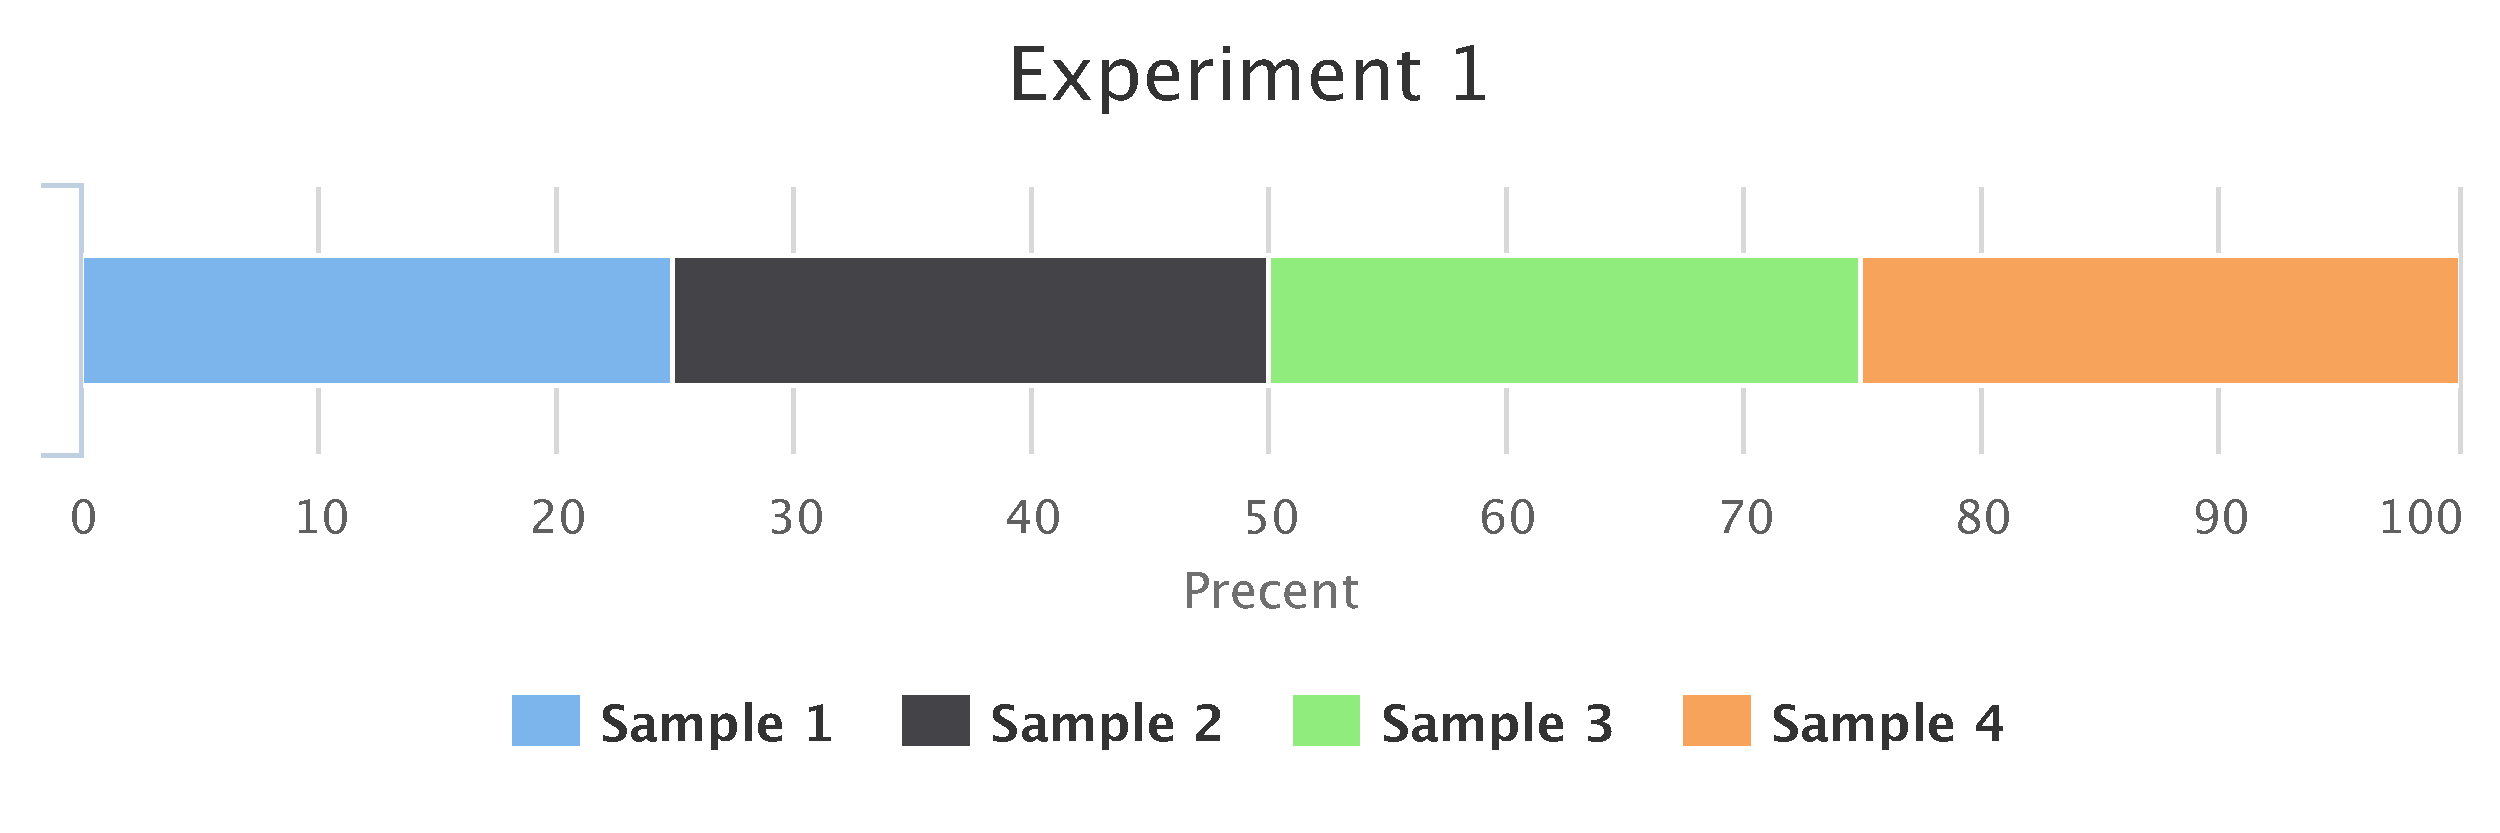
\includegraphics[width=1.0\textwidth]{images/exp_1_data}
%     \caption{Experiment 1 Data Sample Range}
%     \label{fig:exp_1_data_range}
% \end{figure}

%\subsection{Experiment 2}

% TODO show results
%To address the fixed data sampling used previously random sampling was employed. The number of samples $n$ was not changed from the first experiment. The prediction results improved slightly. The \gls{svm} model also reported an error relating to \textit{max number of iterations reached}. This error indicates that the \gls{svm} model is having trouble effectively separating the two categorizations of data into two distinct sets. Such warnings could mean that the features used for training the model are not linearly separable.

% TODO show a picture of how the data was divided.

% \subsection{Experiment 3}

% % TODO talk about using easy.py
% Further investigation into \gls{svm} lead to a research tool that provided grid search for optimizing the parameters used for a \gls{svm}. The results of these experiments offered improvements over the previous, however required a long time to find the right parameters and works the best with the dataset $data_i$ that was used to find the parameters.

% \subsection{Experiment 4}

% % TODO get experiment results
% Modified the candidate features set to test the \gls{svm} with. Added ones like change frequency, average time between commits, number of commits since last change, time since last change and previous change type. Dropped commit author in favor of using just committer. Finally changed the prediction to predict the whether a change will occur within the next 5 commits. In terms of the methodology, 2 variations were tested. The first one was predicting changes to a methods within the same package. The second one was prediction changes to a method within the same file. Neither of these changes provided substantial improvements since they reduced the available sample size, $|data_i|$, down so that the no reasonable predictions could be made from the reduced set.

% \subsection{Experiment 5}

% The next set of experiments required more complex features which necessitated more complex queries from the database. In fact the database interface in use, MySQL, was unable to implement some of the queries. MySQL only allows 2 levels of nested queries and has a more restrictive data type set. An alternative database interface PostgreSQL was used as a replacement for MySQL. PostgreSQL offers fair more sophisticated data types as well as \gls{cte}. The migration from MySQL to PostgreSQL was simplified through the use of pgloader as mentioned in \autoref{sec:storage}. 

% Another change was the even out the number of samples collected from each category. The data set $data_i$ tended to provide unbalanced categorization of the data. The same number of samples from each $n/2$ was collected to prevent biasing in the data set. A \gls{svm} model like most other machine learning algorithms is susceptible to category biasing. This will occur when the training set consists of $80\%$ of one category and $20\%$ of another. The model will train such that it always predicts the first category. This works out well if the data is always unbalanced in the same way however it will fail to predict the smaller category entirely. Therefore providing an even sample of each category ($50\%$ each) will prevent poor prediction results.

% Another result of determining that the data set was unbalanced in terms of the categorization was to calculate both precision and recall of the results. Accuracy alone only provides a very simple measure of how well the model predicted the samples from $data_{i+1}$. A clearer understanding is available with these three measures. Also with each provided an attempt can be made to optimize all three.

% Finally the last few tests in this experiment set included a new feature. This feature was the difference in time between the previous commit with a change and the latest commit. This feature was not particularly useful however and caused the data to become inseparable.

% At the end of this set of tests it was apparent that a deeper understanding of the candidate features was necessary to improve the results. Therefore an analysis of each candidate feature was performed both on the quality of the feature and the possible relationship with others. \gls{svm} models are particularly sensitive towards dependencies between the variables. It was also necessary to properly convert data into a format that could be used by the database. This was talked about in more detail in \autoref{subsec:svm_prediction}.

% \begin{table}
% \begin{center}
%     \begin{tabular}{|l|l|l|}
%         \hline
%         Project & Sample Size (n) & Accuracy \\
%         \hline  
%         acra & 100 & $70\%$ \\
%         acra & 1000 & $52\%$ \\
%         \hline
%     \end{tabular}
% \end{center}
%     \caption{Experiment 5 Results}
%     \label{tab:experiment_5_results}
% \end{table}

% \subsection{Experiment 6}

% After analyzing the candidate features a more ideal set of features was created. The tests were preformed again using sample sizes of $100$ and $1000$. After the changes were made to the data, the performance improved however some of the features did not prove as useful. However the improvement was marginal and therefore necessitated shift in focus from the features to the prediction method. Specificity the data sampling method was inspected to attempt improve the prediction results. Instead of breaking the data set into four even sets based on the date range the data was divided into two even sets based on date as shown in \autoref{fig:exp_6_data_range}

% \begin{figure}[!ht]
%     \centering
%         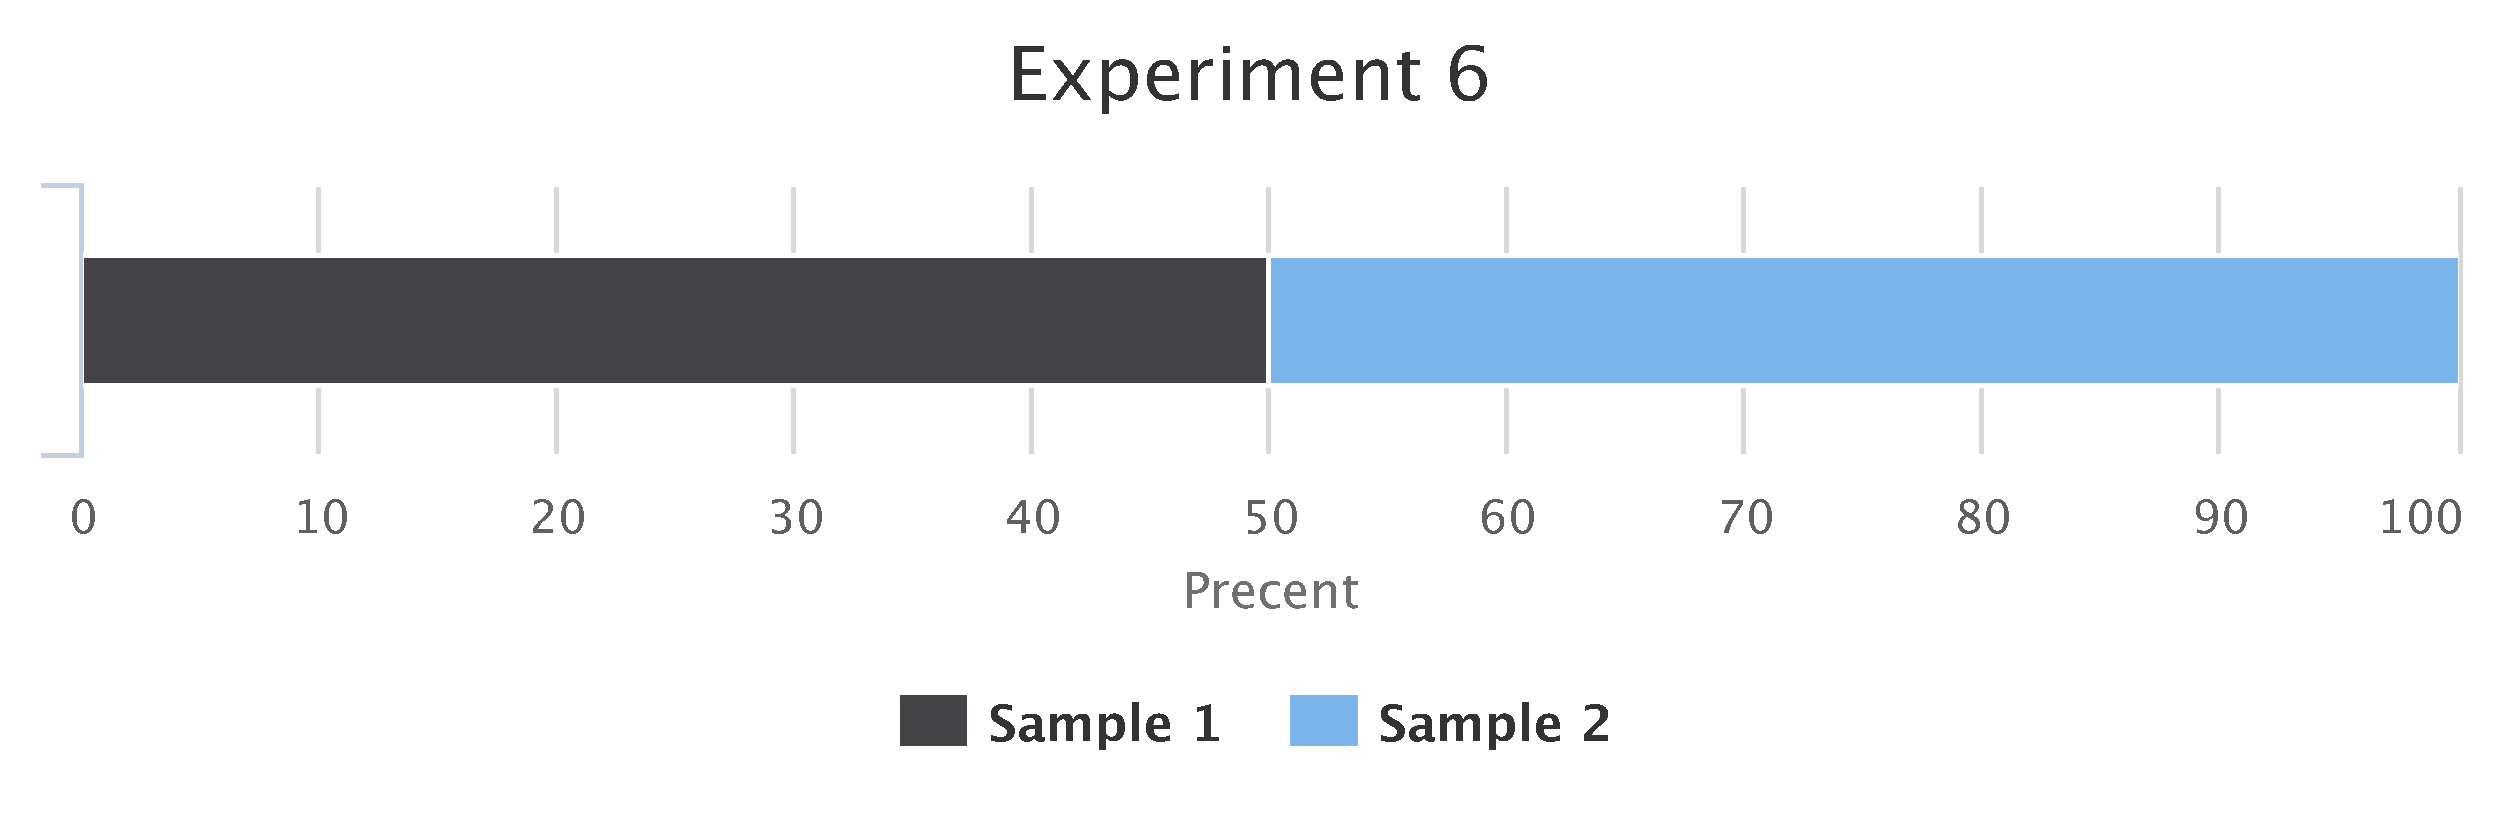
\includegraphics[width=1.0\textwidth]{images/exp_6_data_range}
%     \caption{Experiment 6 Data Sample Range}
%     \label{fig:exp_6_data_range}
% \end{figure}

%The results of the experiment are outlined in \autoref{tab:experiment_6_results}. The larger sample with $n = 1000$ is far worse than with $n = 100$. This however was a worse result than when the data set was divided into 4 equal parts.

% \begin{table}
% \begin{center}
%     \begin{tabular}{|l|l|l|}
%         \hline
%         Project & Sample Size (n) & Accuracy \\
%         \hline
%         acra & 100 & $60\%$ \\
%         acra & 1000 & $47\%$ \\
%         \hline
%     \end{tabular}
% \end{center}
%     \caption{Experiment 6 Results}
%     \label{tab:experiment_6_results}
% \end{table}

% \subsection{Experiment 7}

% Reorganized the data sampling method to sample based on commit ranges rather than date ranges. Instead of splitting the data set into four even sections, the sample range is taken from the current commit $c_i$ to $c_{i-m}$ in the case that $i > m$. $m$ denotes the width in commits of the sample space. For example if the model is predict a change that occurs within the next 5 commits and $m = 30$ then \autoref{fig:data_range} shows how the data would be sampled. The training sample would be where data would be collected from to train the model. The prediction gap is to account for the data sampling calculating whether methods at commit 40 will have a change within the next 5 commits. Therefore to properly test it on data that is not used as part of the testing model the offset is needed. The testing sampling section is the same size as the training sampling data set and follows the 5 commit gap.

% \begin{figure}[!ht]
%     \centering
%         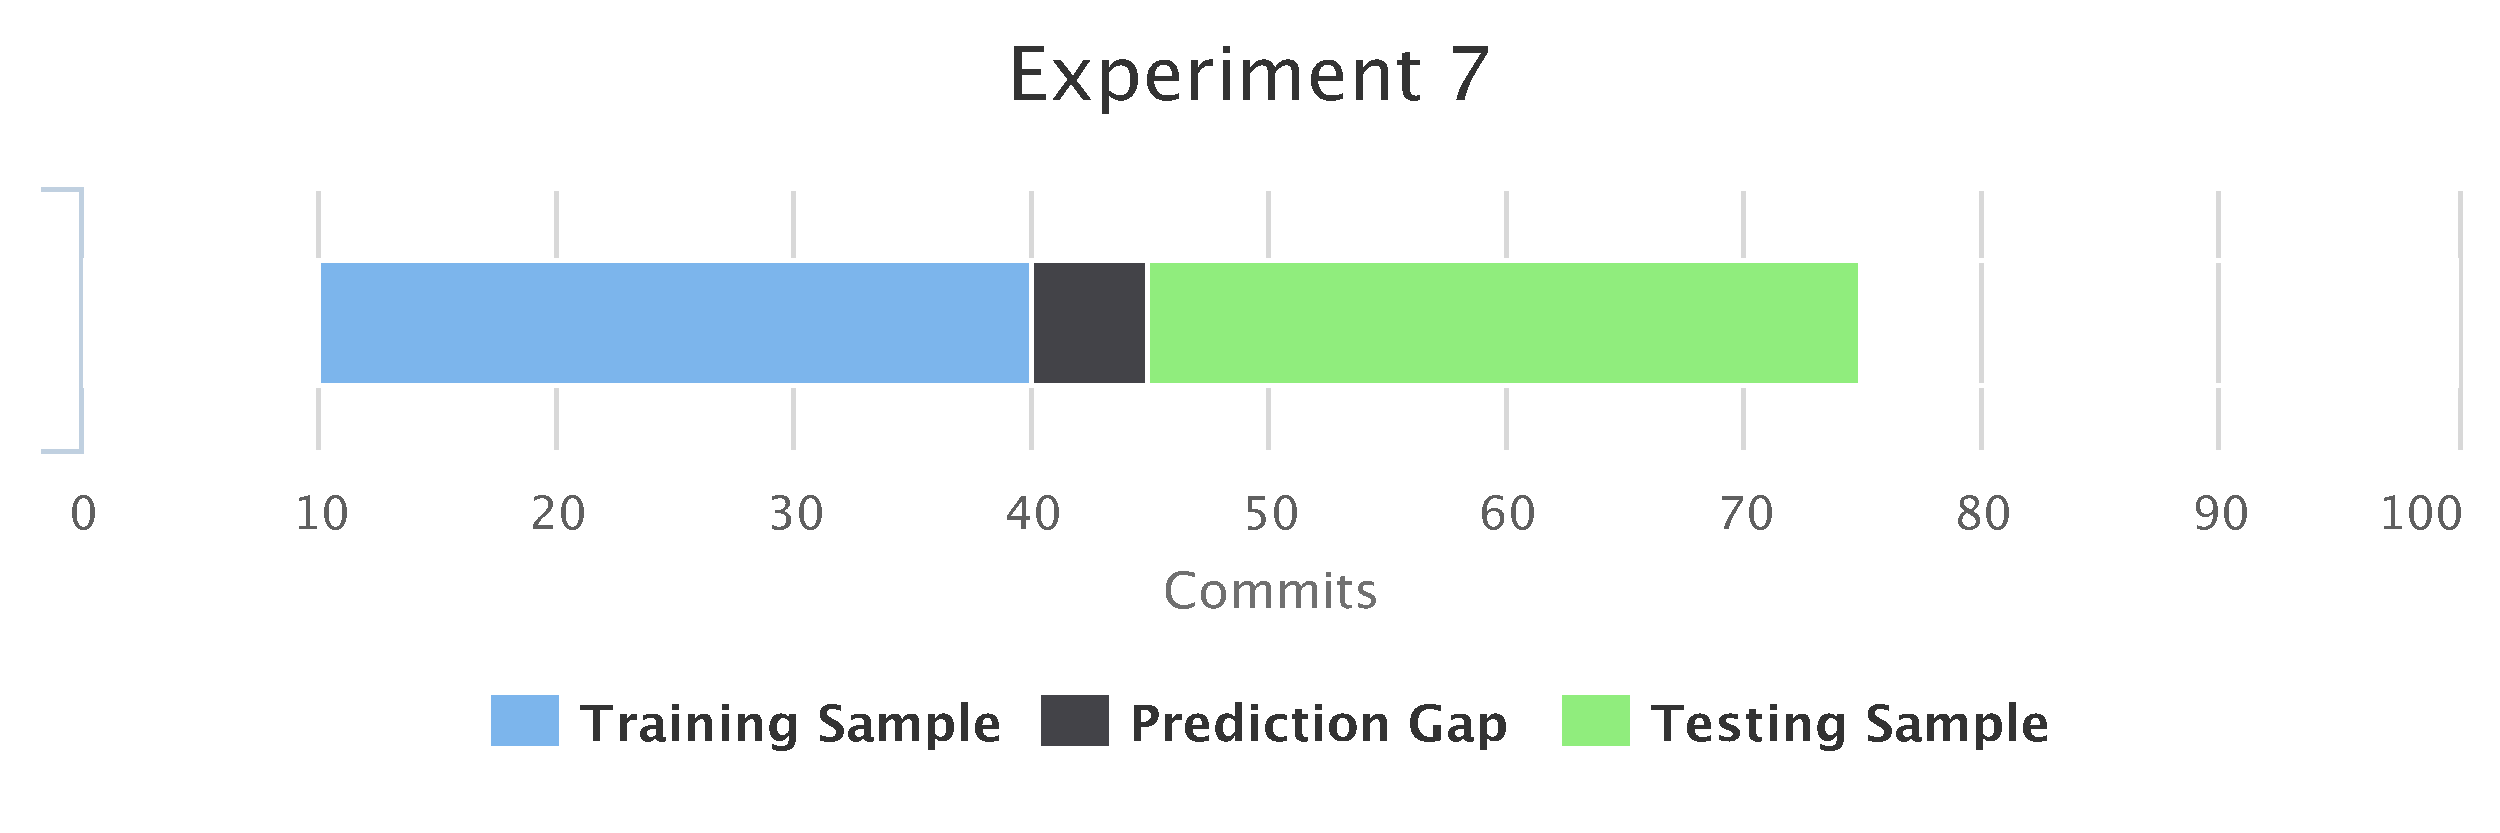
\includegraphics[width=1.0\textwidth]{images/exp_7_data_range}
%     \caption{Experiment 7 Data Sample Range}
%     \label{fig:data_range}
% \end{figure}

% Another change to the sampling method was to sample a percentage of the data within the sample rather than a fixed amount. The sample ranges provided a larger range of data to sample and thus sticking to a arbitrary amount of tuples was updated. This however introduced biasing issues with the data set since typically one category or the other had the majority of tuples within the sample. Fixing this issue is talked about in further detail in \autoref{subsec:random_forest_predictions}. Similar to the previous sampling techniques the data set was sampled randomly. Therefore the percentage of data sampled had a large impact on how long it took to train the model but typically also on the prediction results of the model. 

% TODO discuss the results

% \subsection{Experiment 8}

% After more or less establishing a data sampling model the candidate feature set was looked at again in an attempt to improve the prediction results. A few of the candidate features were removed and a minimum candidate feature set was determined which provided the best results for the current test project \textit{acra}.

% % TODO show some results

% % TODO outline the candidate feature set that performed the best for SVM

% The optimal value of $m$ is a more challenging issue since for project which have a large amount of rapid change occurring in the project larger value seems to provide a more positive result. Where as smaller projects or ones that have a slower rate of change tend to do far better with a smaller value of $m$. 

% \subsection{Experiment 9}

% After the results of the previous experiments proved to less consistent for other data sets such as \textit{storm} and \textit{fresco} another prediction algorithm was tested. \gls{rf} as discussed in greater detail in \autoref{subsec:random_forest_predictions} is more capable with unbalanced datasets and is generally more widely used for performing predictions on mined data. % TODO cite this.

% \gls{rf} while proving to be at times easier to get better results also had some of the challenges that the \gls{svm} model experienced. For example the best features to use in the prediction model and also the best commit width ($m$) to optimize the results.

\section{Experimental Setup}

\subsection{Prediction Features}

%The experimental process for testing the various feature sets on acra involved dividing the repository into four equal quarters (based on time duration). While the number of commits within each period may vary greatly, only a sample is taken.

    %- Alternatively the periods could be distributed such to make the number of commits equal between the sections. Further testing is needed to determine which method is more ideal.

%The \gls{svm} model was trained to categorize whether the current method would be changed within the next 5 commits. This of course can generalize to whether a vector will have a commit within the next \textit{n} commits. Obviously each candidate feature leverages historical or current information and thus a vector can be generated without future information.

%238, ReportField.java            |           8234 | public boolean getValue() {                                                                          |           0 | william-ferguson-au |  0.0464135021097046 | ("{3,3,0,0,0}","{68,1816,549469,779372,208198}")                              |        0
% TODO update this list based on new candidates
\begin{table}
\begin{center}
    \begin{tabularx}{\linewidth}{|l|X|l|l|}
        \hline
        Feature & Description & Data & Example Vector \\
        \hline
        $name$ & The name of the file & Main.java & 3 \\ \hline
        $signature$ & The method name related to the change details & void work() \{ & 46\\ \hline
        $change_i$ & Whether the method changed or not at the current commit & 3 & 1 \\ \hline
        $committer$ & The individual who committed the change & bob & 5 \\ \hline
        $freq_{change}$ & The number of changes this method has been involved divided by the number of commits up till this point & 0.0464 & 0.0464 \\ \hline
        $change_{prev}$ & A list of whether the method changed or not for the last 5 commits & \{3,3,0,3,1\} & \{1,1,0,1,1\} \\ \hline
        $\Delta t$ & A set of time deltas between the last 5 commits that involved the method & \{68,416,569,772,898\} & \{68,416,569,772,898\} \\
        \hline
        $change_{next\_6}$ & Identifies whether at least one change occurred within the next 5 commits for the given method & 0 & 0\\
        \hline
    \end{tabularx}
\end{center}
    \caption{Candidate features for \gls{svm} model}
    \label{tab:candidate_features}
\end{table}
%& \{68,1816,5469,7772,8198\} 

% Name => Methods within a file are likely going to have similar change patterns
% Signature => A method change history will likely be unique
% Change_i => Whether the method changed or not at the current commit may provide insight as to whether the next 5 commits will feature a change as well.
% committer => Users may change in different change patterns thus helping identify whether this will be a change or not, 
% freq_change => Helps identify how likely the file is to change

The \autoref{tab:candidate_features} lists each feature with a more detailed description. An example of each feature is provided to further illustrate them. As stated in the previous \autoref{subsec:svm_prediction}, the values need to be first converted into floating point numbers. First the data is extracted from the database as \textit{raw} values as shown in the \textit{\textbf{Data}} column. Taking the $name$ value, ``Main.java'' will be mapped to the value 3. This is because 2 other methods have already been mapped and therefore method name is mapped to the next available mapping, 3. Similarly both $signature$ and $committer$ will be mapped from their respective values ``void work() \{'' and ``bob'' to 46 and 5. Numerical values are easily converted by casting them to floating point values if they are not already of that type. For spacing reasons all the values in the table that were integers to begin are shown without a ``.0''following.

Another small change made to the data to create a vector for the \gls{svm} model was to apply \autoref{eq:change_type} to the values of $change_i$ and $change_{prev}$. As in \autoref{tab:candidate_features}, the value of $change_i$ is initially 3 which indicates a modification occurred. Since a modification is a type of change $C(change_i) = 1$ which is the value used by the vector. Likewise this is also applied to each entry in the $change_{prev}$ changing it into a bit vector.

\begin{equation} 
\label{eq:change_type}
C = \left\{\begin{matrix}
1 & \text{if} change > 0 \\
0 & \text{otherwise}
\end{matrix}\right.
\end{equation}

Both $change_{prev}$ and $\Delta t$ are actually each 5 features since they are a set of features. $change_{prev}$ shows the type of change that occurred for the last 5 commits. Similarly $\Delta t$ shows the difference between the current commit time ($t(c_i)$) and the previous commit time ($t(c_{i-1})$) calculated in \autoref{eq:time_delta}. These two features then expanded to add a new category for each entry in the set. The ordering is maintained since each entry maps to a previous commit in order.

\begin{equation}
\label{eq:time_delta}
\Delta t_{i} = t(c_i) - t(c_{i-1}), i > 1
\end{equation}

% TODO place in a better spot.
$freq_{change}$ is calculated as by taking the number commits which involve changes to the current method ($c_i$) divided by the current number of commits ($c_{cur}$).
\begin{equation}
\label{eq:freq_change}
freq_{change} = \frac{|c_i|}{|c_{cur}|}
\end{equation}

% TODO provide how to calculate the other features.

%TODO write algorithm for mapping names

% TODO put this into the subsection experiment 8-9
Another issue that was necessary to address was the arbitrary sample size. For projects that are a lot bigger 100 vectors which map to 100 method changes could be very small. The sampling also seemed like a peculiar approach to picking the data since it would randomly pick values from over a period that could vary from a few months to a few years depending on the size. Therefore instead of dividing the project into four quarters based on time a number of commits is picked. The test is then designed around a given date with the \textit{gap} with $t$ and $p$ commits proceeding it as the range of the test. $t$ is the number of commits that the training dataset will sample from. Alternatively, $p$ is the number of commits that the testing dataset will sample from. In the case that $t = p$ the training commit size and the testing commit size are the same.

The final change that was accounted for was to change the population sample size from a fixed number to a percentage. This allows more flexibility and determining the sample size of a test by allowing for it to scale based on the size of the project. 

% TODO show a final picture with population size as a percentage.

% TODO access this stuff below. Remember It's now 5 commits not 6 and also a lot of this stuff is no longer relevant.

The initial thought was to provide a few different features that appeared to be unique and potentially provided useful information for whether the method will change within the next 5 commits. Of course since this measurement is calculated, if a vector within the sample set is within the last 5 commits then it will leverage data from the next quarter to provide its prediction. This has not been mitigated and could provide a unrealistic improvement in the prediction score if members of the next sample fall into the first 5 commits. The way to mitigate this would be to provide a buffer between the two sets when the second test is used for testing purposes. The second set would be restricted further, such that the changes must come from after the 6th commit from the start date of the quarter. The first commit would be the one that takes place on or right after (if no commit falls on that date) the start date. The next 5 commits would also be excluded from the test sample set.

\subsection{Experiment Factors}
% TODO outline the different factors used in the experiments. Also even outline other factors that are not changed either.

% Factors:
% Sliding Window
% Extended sampling ranges
% Training Range
% Testing Range
% Sample Range by Commit (or by date)
% Oversampling
% Undersampling
% Dynamic Size of sampling
% Sampling Percent
% Sampling Randomly
% Window
% SVM or Forest Parameters

Reorganized the data sampling method to sample based on commit ranges rather than date ranges. Instead of splitting the data set into four even sections, the sample range is taken from the current commit $c_i$ to $c_{i-m}$ in the case that $i > m$. $m$ denotes the width in commits of the sample space. For example if the model is predict a change that occurs within the next 5 commits and $m = 30$ then \autoref{fig:data_range} shows how the data would be sampled. The training sample would be where data would be collected from to train the model. The prediction gap is to account for the data sampling calculating whether methods at commit 40 will have a change within the next 5 commits. Therefore to properly test it on data that is not used as part of the testing model the offset is needed. The testing sampling section is the same size as the training sampling data set and follows the 5 commit gap.

\begin{figure}[!ht]
    \centering
        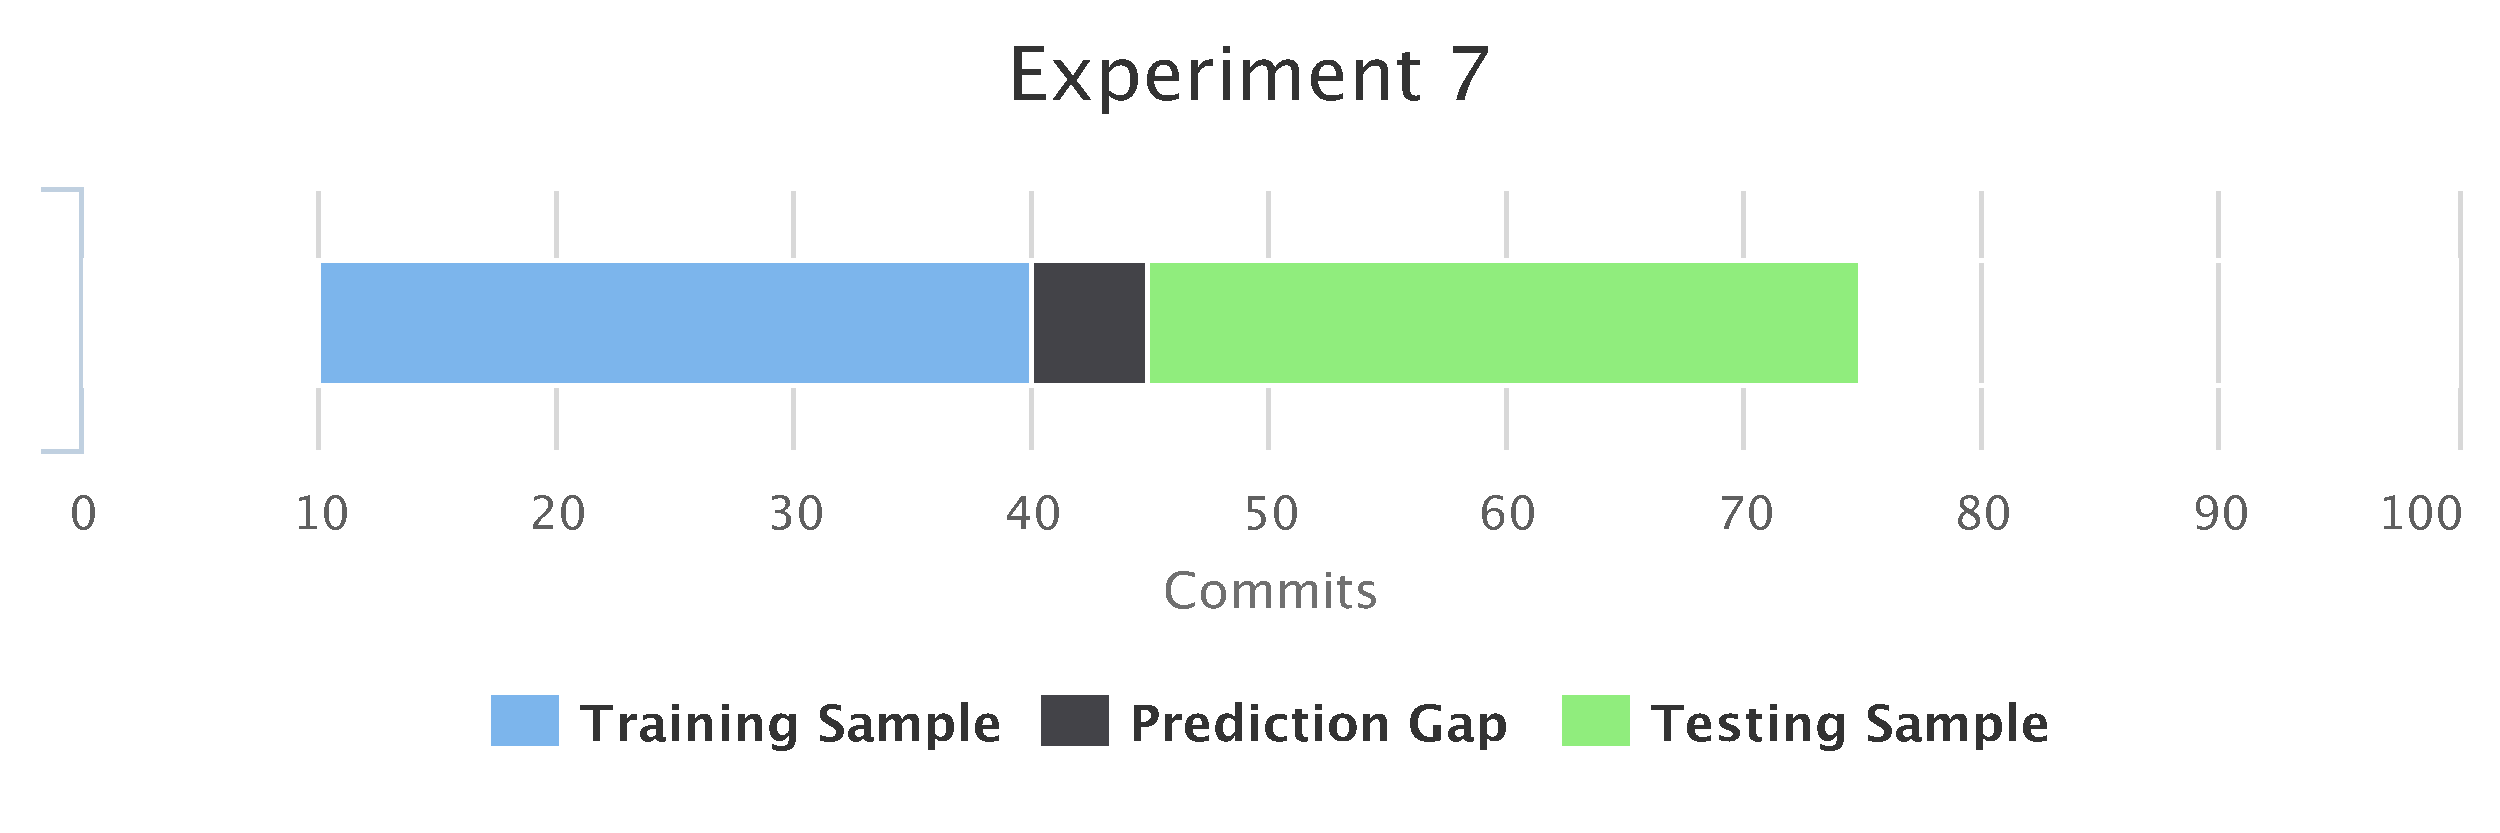
\includegraphics[width=1.0\textwidth]{images/exp_7_data_range}
    \caption{Experiment 7 Data Sample Range}
    \label{fig:data_range}
\end{figure}

The sliding window factor is one of core aspects related to extracting samples from the data set. When using the sliding window to sample the data the data is divided as shown in \autoref{fig:data_range}. The training sample is where the training data set is sampled from. The testing sample is where the testing data is sampled from. 

A data set with an extended sampling range will extend the sampling range beyond the original size for either the training sample or the testing sample. The training range can be expanded to include earlier samples to increase the sample space.

The training and testing sampling range are defined as the number of commits from which the samples can be taken. In \autoref{fig:data_range}, both the training and testing sample ranges are set to 30 commits. These two values can differ from one another but tend to be kept the same for most of the experiments.

Two other factors in the experiments was handling the data set bias. The two methods are oversampling and undersampling of data elements. Most of the time a data set will contain more samples in one category than the other. When the number of samples in each category is very close this will have little effect on the model. However in cases were the data is highly skewed to one classification over the other the model will simply predict the larger classification. Use of oversampling will take more samples (duplicates) from the smaller classification to be closer in size to the larger classification. Alternatively, undersampling will use remove samples from the larger classification to become closer in size to the smaller classification.
% Discussed further in section in approach

Another feature assessed was that of the sample size. The sample size was determined by the sample ratio. When sampling if the ratio is at 50 \% then only half of the values retrieved will be used to train or test. For some of the larger data sets sampling 100 \% of the data from the range would take a lot longer. Therefore sampling a percentage of the data set is commonly used to decrease the training time. However in the case of using a percentage of the sample range the data should to be sampled randomly to provide a more stable model. Therefore each data entry in the sample has the same chance to be within the training or test data set.

For each project data set there are numerous windows that be can be used. The window number is setting which window is used broadly mapping to the position within the data set that the model will be trained on and then predicted on. As shown in \autoref{fig:data_range}, the window is shown starting at the 30th commit which would also be called the 30th window.

Finally, the last factor of note is the parameters used to configure each prediction method. \gls{rf} use a single parameter, the size of the forest. \gls{svm} meanwhile uses three parameters; C, gamma and esp. % TODO explain each of them in a bit more details.

\subsection{Prediction Performance}

% TODO this isn't necessary for cases when the entire sample is used.
For each experiment where the used random sampling the experiment was performed 5 times to account for variations in the random sample. Therefore if the initial results using the first sample set were not characteristic of the full dataset then running the experiment with more random samples is more likely to represent the true characteristics of the dataset. This required taking five random samples from each quarter, training the model and running the tests on the model to then determine the average prediction score. In the case when $100\%$ of the sample is used then only one sample is is taken since there will be no variations within the sample set.

The goal of the prediction methods are to provide a good prediction of whether the a given vector will fit in one category or the other. A model's prediction performance can be rated using three measures of accuracy, precision and recall. Accuracy is measured as how often predictions $p$ are classified correctly where $a_i$ represents vector $v_i$ correct classification. The algorithm for calculating a single vectors accuracy is showing in \autoref{eq:vector_accuracy}. The prediction accuracy ($P_{accuracy}$) can then be calculated using \autoref{eq:prediction_accuracy}. This simply sums up the accuracy for each vector and then divides it by the total number of vectors (where $n = |v|$).

\begin{equation} 
\label{eq:vector_accuracy}
v_i = \left\{\begin{matrix}
1 & \text{if } p_i = a_i\\ 
0 & \text{otherwise}
\end{matrix}\right.
\end{equation}

\begin{equation}
\label{eq:prediction_accuracy}
P_{accuracy} = \frac{\sum_{i=0}^{n}v_i}{n} \times 100
\end{equation}

The precision of a model is the measure of how correct the model predicts that a change will occur when it predicts that a change will occur. Given the true positives $tp$, represents the number of predictions that the model correctly identified as having a change and the false positives $fp$ is the number of times the model incorrect predicted a change to occur when it in fact did not. The equation for calculating precision is show in \autoref{eq:precision}.

\begin{equation} 
\label{eq:precision}
P_{precision} = \frac{tp}{tp+fp}
\end{equation}

The recall of the model is the measure of how correct the model predicts that change will occur out of all the times changes really occurred. Again using $tp$ as the number of true positives, and false negatives $fn$ which is the number of times the model fails to predict that a change will occur. The recall can be calculated using the \autoref{eq:recall}

\begin{equation} 
\label{eq:recall}
P_{recall} = \frac{tp}{tp+fn}
\end{equation}

\section{\gls{svm} Experiments}
\label{sec:svm_experiments}

The experiment is setup to have a set of parameters that can be set. These parameters will remain constant to observer the difference that the independent variable will have on the dependent variables, precision, recall and accuracy. Each experiments will use one of the parameters as the independent variable. 

\subsection{Window Range Experiments}

%TODO fill out details of experiments

For this experiment the variable was the size of the \gls{swr} in commits. In \autoref{tab:window_range_experiment_features}, the features used by the prediction model are outlined. Features with a mark, $\bullet$, are used while those without are not. In this experiment only the Short $\Delta_{freq}$ is not used while all the rest are.

% TODO use a better way of showing this like a table with dots.
\begin{table}[h]
\begin{center}

    \begin{tabular}{|c|c|c|c|c|c|c|c|}
        \hline
        Com & Sig & Name & $\Delta_{freq}$ & Short & $t_{i} - t_{i-1}$ & Length & Has \\
         & & & & $\Delta_{freq}$ & & & Next \\ \hline
        $\bullet$ & $\bullet$ & $\bullet$ & $\bullet$ & & $\bullet$ & $\bullet$ & $\bullet$ \\ \hline
    \end{tabular}
    \caption{\gls{swr} Experiment Features}
    \label{tab:window_range_experiment_features}
\end{center}

\end{table}

%% TODO create a table to show this information.
% Extend Window: No% Sample by Commit Range: Yes
% Over Sampling: No
% Under Sampling: Yes
% Sample Rate: 100%
% Window Offset: 5
% SVM c: 10
% SVM gamma: 8
% SVM esp: 0.001

As noted above the independent variable for this experiment is the \gls{swr}. The remaining parameters for the experiment are constant for each test. The parameters for this experiment are outlined in \autoref{tab:window_range_experiment_setup}.

\begin{table}[h]
\begin{center}

    \begin{tabular}{|c|c|c|c|c|cc|}
        \hline
        Extended & Over & Under & Sample & Window & SVM & \\
        Window & Sampling & Sampling & Rate & Offset & C & gamma \\ \hline
        No & No & Yes & $100\%$ & 5 & 10 & 8 \\ \hline
    \end{tabular}
    \caption{\gls{swr} Experiment Setup}
    \label{tab:window_range_experiment_setup}
\end{center}

\end{table}

The results for the experiments are shown with the precision, recall and accuracy. For each graph the independent variable is the number of commits in the \gls{swr}. Y-axis is the value of each of the different plot, either precision, recall and accuracy. The first project, acra, in \autoref{fig:test_1_acra_svm} has the strongest performance out of all the projects. The best performance for acra is at \gls{swr} at 80 commits width.

\begin{figure}[h]
    \centering

    \begin{minipage}[b]{0.45\linewidth}
        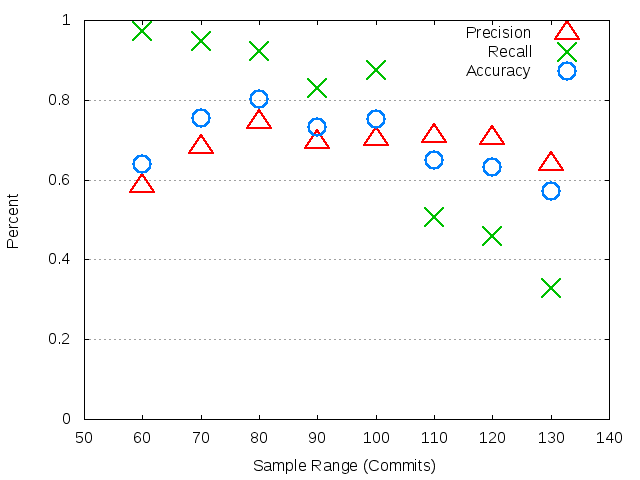
\includegraphics[width=1.0\textwidth]{images/svm/test_1/acra_sample_range}
        \caption{\gls{swr} for acra using \gls{svm}}
        \label{fig:test_1_acra_svm}
    \end{minipage}
\quad
    \begin{minipage}[b]{0.45\linewidth}
        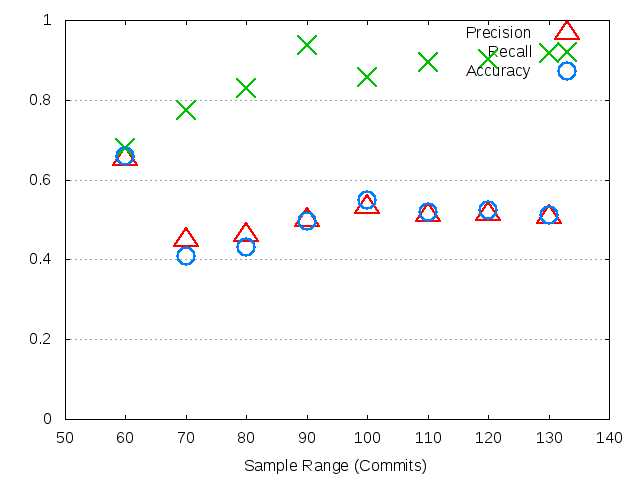
\includegraphics[width=1.0\textwidth]{images/svm/test_1/dagger_sample_range}
        \caption{\gls{swr} for dagger using \gls{svm}}
        \label{fig:test_1_dagger_svm}
    \end{minipage}
\end{figure}

\begin{figure}[h]
    \centering

    \begin{minipage}[b]{0.45\linewidth}
        % add 120, 130
        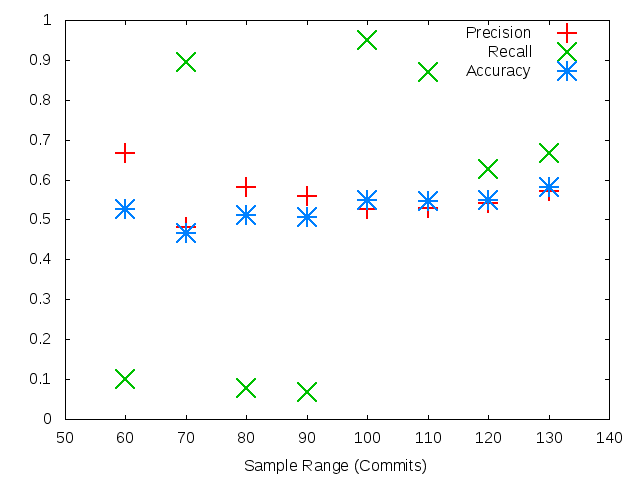
\includegraphics[width=1.0\textwidth]{images/svm/test_1/fresco_sample_range}
        \caption{\gls{swr} for fresco using \gls{svm}}
        \label{fig:test_1_fresco_svm}
    \end{minipage}
\quad
    \begin{minipage}[b]{0.45\linewidth}
        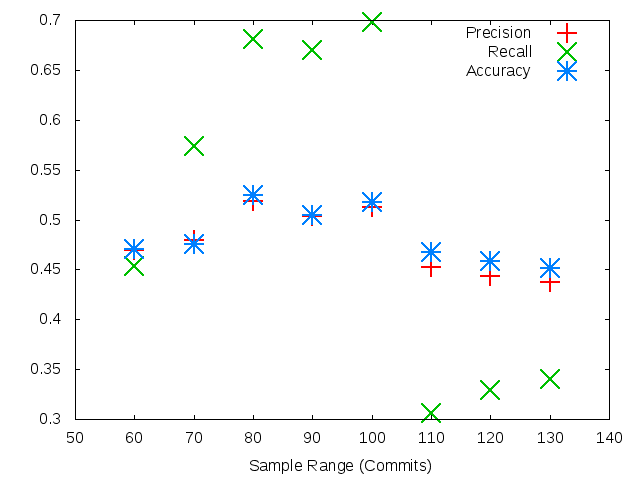
\includegraphics[width=1.0\textwidth]{images/svm/test_1/storm_sample_range}
        \caption{\gls{swr} for storm using \gls{svm}}
        \label{fig:test_1_storm_svm}
    \end{minipage}
\end{figure}

\begin{figure}[h]
    \centering
    %TODO add 130
        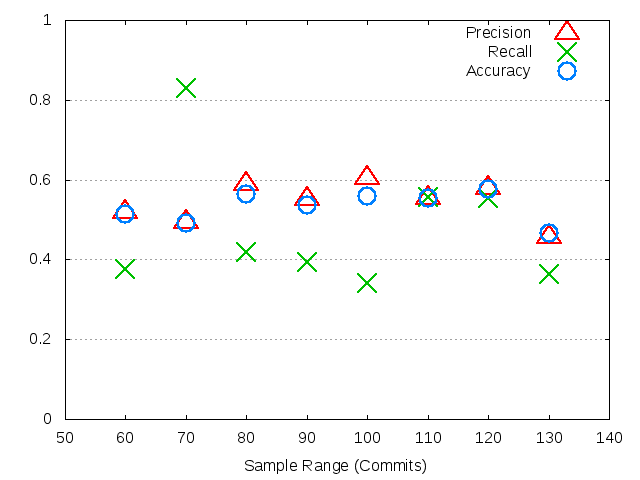
\includegraphics[width=0.45\textwidth]{images/svm/test_1/deeplearning4j_sample_range}
    \caption{\gls{swr} for deeplearning4j using \gls{svm}}
    \label{fig:test_1_deeplearning4j_svm}
\end{figure}

Alternatively, dagger has abysmal performance with the exception of a \gls{swr} of 60. Fresco prediction performance does not particularly differ greatly. Also, it should be noted that the experiments with a \gls{swr} of 120 and 130 since both resulted in a undefined precision and recall of 0 and accuracy of $0.5$.

Apache had slight variations, however the precision and accuracy never exceeded $0.55$. Finally, deeplearning4j does not have very good performance with low recall results. As shown in the plots, the \gls{swr} has a significant impact on the performance of the model. While the actual width varies widely per project, there are projects with a width that fares worse and others that fare far better.

Overall there was no clear value for the \gls{swr} which held consistent positive results. Generally speaking, projects that were smaller; acra, dagger, fresco, appeared to get positive results with smaller windows. Alternatively, larger projects; storm and deeplearning4j both did fairly poorly with the test range from 60 to 130. The largest project, deeplearning4j also has a slight positive trend towards the end of the range. However, storm does have a negative trend towards the end of the range.

The precision and accuracy remain fairly stable throughout this experiment. While the value of these attributes changes with different values of the \gls{swr} these changes tend to be fairly close and follow a general trend. However for dagger in \autoref{fig:test_1_dagger_svm} the performance of accuracy and precision drops from $0.6 - 0.7$ range to $0.4 - 0.45$ range. The accuracy and precision also do however remain rather stable for the remainder of the experiments in this set.

Finally, the recall for the prediction is very unstable. While both accuracy and precision are very closely related and so will be likely close in value. Recall however will vary from a very low value to a very high value. For example in \autoref{fig:test_1_fresco_svm} the value of recall at \gls{swr} of $60$ is $0.1$ and then jumps to $0.9$ at \gls{swr} of $70$. \autoref{fig:test_1_storm_svm} and \autoref{fig:test_1_deeplearning4j_svm} both also have large changes in the recall but none as drastic as shown in fresco. 

% \begin{figure}[!ht]
%     \centering
%         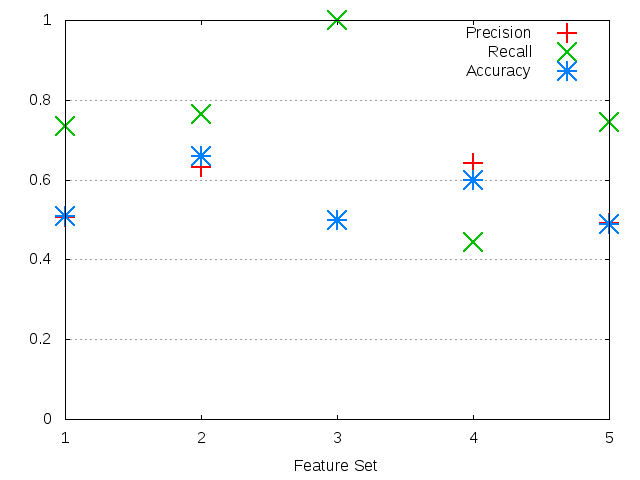
\includegraphics[width=1.0\textwidth]{images/test_1/dagger_sample_range}
%     \caption{\gls{swr} for dagger}
%     \label{fig:test_1_dagger}
% \end{figure}

% \begin{figure}[!ht]
%     \centering
%         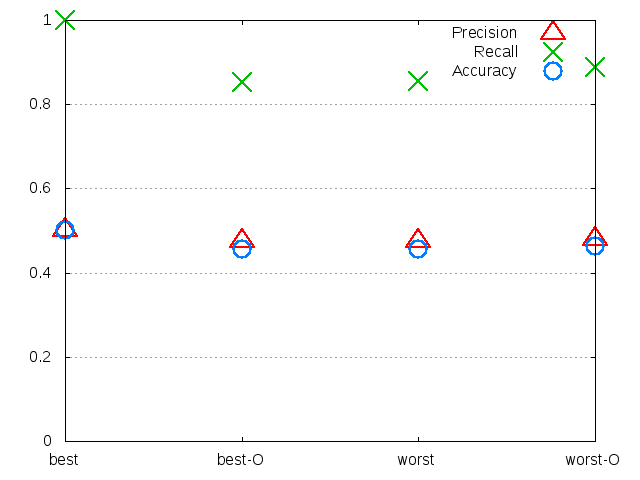
\includegraphics[width=1.0\textwidth]{images/test_1/fresco_sample_range}
%         \caption{\gls{swr} for fresco}
%         \label{fig:test_1_fresco}
% \end{figure}

% \begin{figure}[!ht]
%     \centering
%         \includegraphics[width=1.0\textwidth]{images/test_1/storm_sample_range}
%         \caption{\gls{swr} for storm}
%         \label{fig:test_1_storm}
% \end{figure}

% \subsection{\gls{swr} Experiments 2}

% For this experiment the variable was the size of the \gls{swr} in commits. In \autoref{tab:window_range_experiment_features}, the features used by the prediction model are outlined. Features with a mark, $\bullet$, are used while those without are not. In this experiment only the Short $\Delta_{freq}$ is not used while all the rest are.

% \begin{table}[h]
% \begin{center}

%     \begin{tabular}{|c|c|c|c|c|c|c|c|}
%         \hline
%         Com & Sig & Name & $\Delta_{freq}$ & Short & $t_{i} - t_{i-1}$ & Length & Has \\
%          & & & & $\Delta_{freq}$ & & & Next \\ \hline
%         $\bullet$ & $\bullet$ & $\bullet$ & $\bullet$ & $\bullet$ & & $\bullet$ & $\bullet$ \\ \hline
%     \end{tabular}
%     \caption{Window Range Experiment Features}
%     \label{tab:window_range_experiment_features}
% \end{center}

% \end{table}

% %% TODO create a table to show this information.
% % Extend Window: No% Sample by Commit Range: Yes
% % Over Sampling: No
% % Under Sampling: Yes
% % Sample Rate: 100%
% % Window Offset: 5
% % SVM c: 10
% % SVM gamma: 8
% % SVM esp: 0.001

% As noted above the independent variable for this experiment is the \gls{swr}. The remaining parameters for the experiment are constant for each test. The parameters for this experiment are outlined in \autoref{tab:window_range_experiment_setup}.

% \begin{table}[h]
% \begin{center}

%     \begin{tabular}{|c|c|c|c|c|cc|}
%         \hline
%         Extended & Over & Under & Sample & Window & SVM & \\
%         Window & Sampling & Sampling & Rate & Offset & C & gamma \\ \hline
%         No & No & Yes & $100\%$ & 5 & 10 & 8 \\ \hline
%     \end{tabular}
%     \caption{Window Range Experiment Setup}
%     \label{tab:window_range_experiment_setup}
% \end{center}

% \end{table}

% % TODO talk about results

% \begin{figure}[!ht]
%     \centering

%     \begin{minipage}[b]{0.45\linewidth}
%         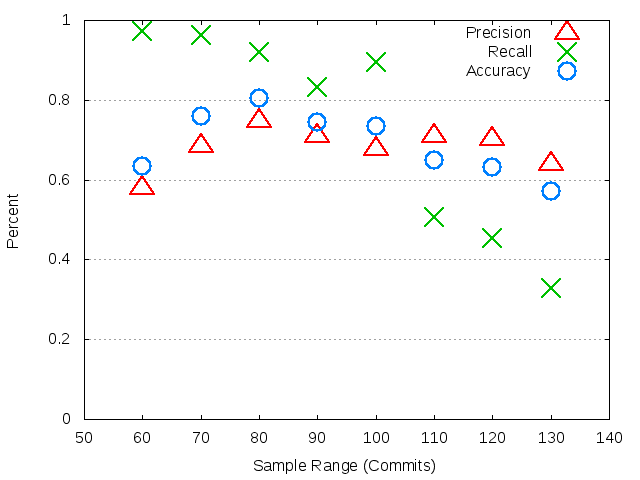
\includegraphics[width=1.0\textwidth]{images/svm/test_2/acra_sample_range}
%         \caption{\gls{swr} for acra}
%         \label{fig:test_2_acra}
%     \end{minipage}
% \quad
%     \begin{minipage}[b]{0.45\linewidth}
%         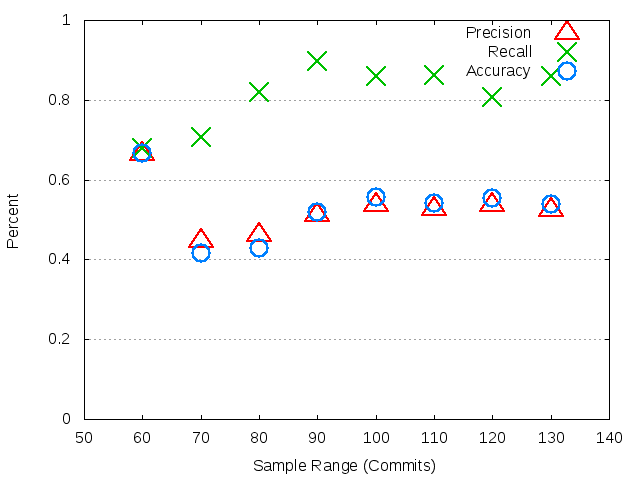
\includegraphics[width=1.0\textwidth]{images/svm/test_2/dagger_sample_range}
%         \caption{\gls{swr} for dagger}
%         \label{fig:test_2_dagger}
%     \end{minipage}
% \end{figure}

% \begin{figure}[!ht]
%     \centering

%     \begin{minipage}[b]{0.45\linewidth}
%         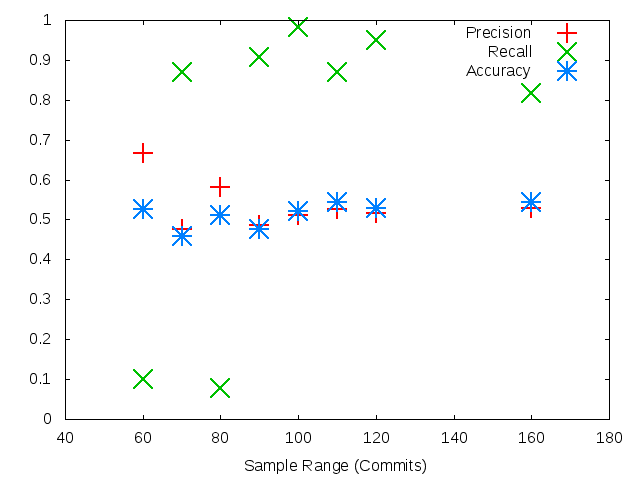
\includegraphics[width=1.0\textwidth]{images/svm/test_2/fresco_sample_range}
%         \caption{\gls{swr} for fresco}
%         \label{fig:test_2_fresco}
%     \end{minipage}
% \quad
%     \begin{minipage}[b]{0.45\linewidth}
%         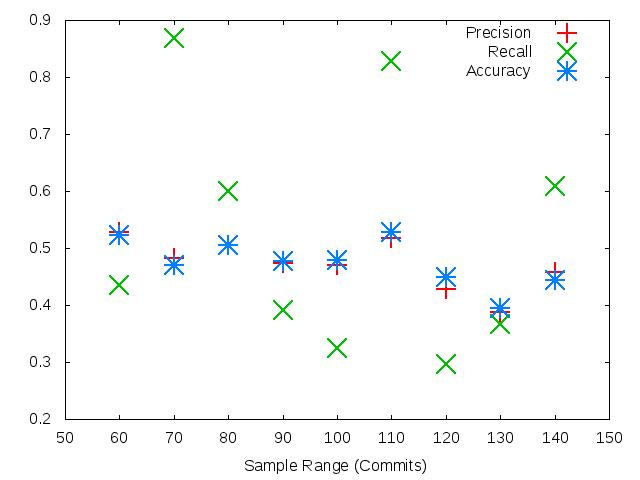
\includegraphics[width=1.0\textwidth]{images/svm/test_2/storm_sample_range}
%         \caption{\gls{swr} for storm}
%         \label{fig:test_2_storm}
%     \end{minipage}
% \end{figure}

% \begin{figure}[!ht]
%     \centering
%         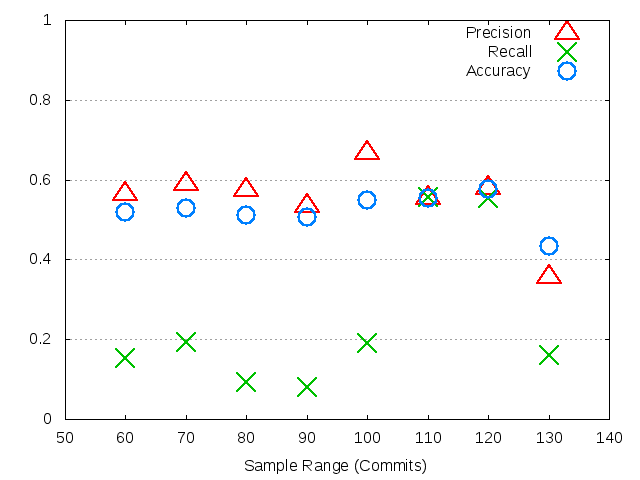
\includegraphics[width=0.45\textwidth]{images/svm/test_2/deeplearning4j_sample_range}
%     \caption{\gls{swr} for deeplearning4j}
%     \label{fig:test_2_deeplearning4j}
% \end{figure}



% TODO add a few more experiments.

\subsection{SVM Discussion}
\label{subsec:svm_discussion}

\section{Random Forest Experiments}
\label{sec:rf_experiments}

\subsection{Factor}

\subsection{Window Range Experiments}

The independent variable for this set of experiments is the sample window size measured in commits. The candidate features are outlined in \autoref{tab:window_range_experiment_features}. Is the same as the first \gls{svm} experiment the candidate feature set.

\begin{table}[h]
\begin{center}

    \begin{tabular}{|c|c|c|c|c|c|c|c|}
        \hline
        Com & Sig & Name & $\Delta_{freq}$ & Short & $t_{i} - t_{i-1}$ & Length & Has \\
         & & & & $\Delta_{freq}$ & & & Next \\ \hline
        $\bullet$ & $\bullet$ & $\bullet$ & $\bullet$ & & $\bullet$ & $\bullet$ & $\bullet$ \\ \hline
    \end{tabular}
    \caption{\gls{swr} Experiment Features}
    \label{tab:rf_window_range_experiment_features}
\end{center}

\end{table}

%% TODO create a table to show this information.
% Extend Window: No% Sample by Commit Range: Yes
% Over Sampling: No
% Under Sampling: Yes
% Sample Rate: 100%
% Window Offset: 5
% SVM c: 10
% SVM gamma: 8
% SVM esp: 0.001

The parameter for this experiment are outlined in \autoref{tab:window_range_experiment_setup}. The major difference between the \gls{svm} and this experiment, \gls{rf}, is the parameters used for the \gls{rf}. This allows for a fairly clear comparison between these two methods with the given independent variable, sample window size.

\begin{table}[h]
\begin{center}

    \begin{tabular}{|c|c|c|c|c|c|}
        \hline
        Extended & Over & Under & Sample & Window & \gls{rf} \\
        Window & Sampling & Sampling & Rate & Offset & Size \\ \hline
        No & No & Yes & $100\%$ & 5 & 10000 \\ \hline
    \end{tabular}
    \caption{\gls{swr} Experiment Setup}
    \label{tab:window_range_experiment_setup}
\end{center}

\end{table}

The results for the experiments with the independent variable sample window size using random forest were mixed. Both acra in \autoref{fig:test_1_acra_rf} and dagger in \autoref{fig:test_1_dagger_rf} have strong prediction results. While the remainder of the projects; fresco in \autoref{fig:test_1_fresco_rf}, storm in \autoref{fig:test_1_storm_rf} and deeplearning4j in \autoref{fig:test_1_deeplearning4j_rf} did not perform as well. While the accuracy and precision were lower, the recall was very high.

\begin{figure}[h]
    \centering

    \begin{minipage}[b]{0.45\linewidth}
        % TODO add 130
        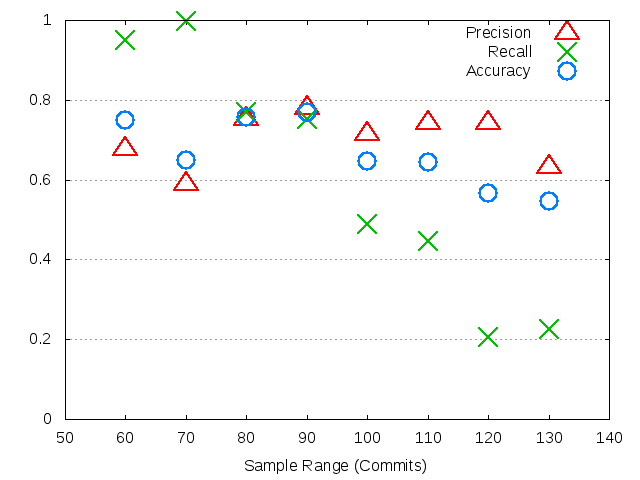
\includegraphics[width=1.0\textwidth]{images/rf/test_1/acra_sample_range}
        \caption{\gls{swr} for acra using \gls{rf}}
        \label{fig:test_1_acra_rf}
    \end{minipage}
\quad
    \begin{minipage}[b]{0.45\linewidth}
        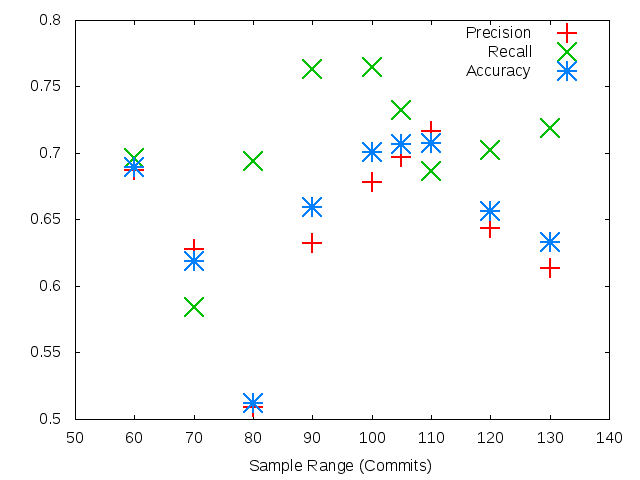
\includegraphics[width=1.0\textwidth]{images/rf/test_1/dagger_sample_range}
        \caption{\gls{swr} for dagger using \gls{rf}}
        \label{fig:test_1_dagger_rf}
    \end{minipage}
\end{figure}

\begin{figure}[h]
    \centering

    \begin{minipage}[b]{0.45\linewidth}
        % TODO add 60
        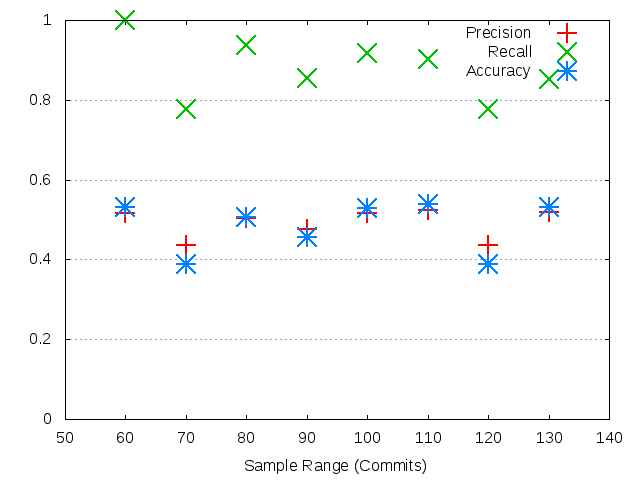
\includegraphics[width=1.0\textwidth]{images/rf/test_1/fresco_sample_range}
        \caption{\gls{swr} for fresco using \gls{rf}}
        \label{fig:test_1_fresco_rf}
    \end{minipage}
\quad
    \begin{minipage}[b]{0.45\linewidth}
        % TODO add 60
        \includegraphics[width=1.0\textwidth]{images/rf/test_1/storm_sample_range}
        \caption{\gls{swr} for storm using \gls{rf}}
        \label{fig:test_1_storm_rf}
    \end{minipage}
\end{figure}

\begin{figure}[h]
    \centering
        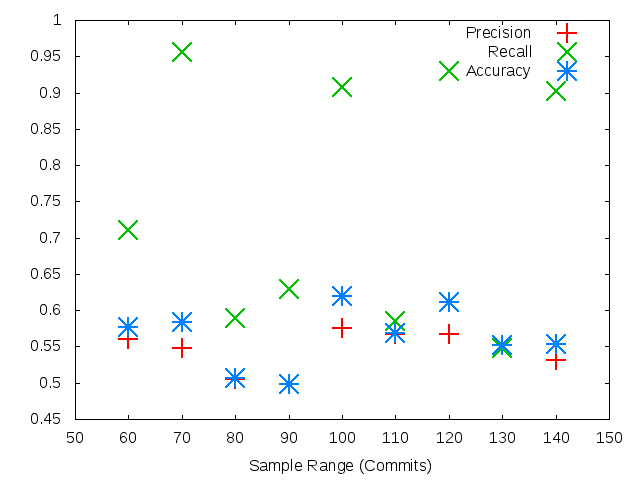
\includegraphics[width=0.45\textwidth]{images/rf/test_1/deeplearning4j_sample_range}
    \caption{\gls{swr} for deeplearning4j using \gls{rf}}
    \label{fig:test_1_deeplearning4j_rf}
\end{figure}


\subsection{Random Forest Discussion}
\label{subsec:rf_discussion}

%\section{Results}

% TODO re-work this section
% TODO most of this section is out of date and needs to be done.


%%%%%%%%%%%%
% This part is fine.

% Ensure this doesn't overlap to much with the above section which discusses cross-validation.

% TODO remove
%Since the data set is split into four quarters, the category (of whether a method will be changed in the next 5 commits) is known for the first 3 quarters. The final quarter depending on the size the category is also known except for the changes that occur in the last 5 commits. Therefore at project testing data set can be extracted using the feature data and the category for each quarter (except for the last 5 commits of the 4th quarter). One extracted the model can be trained on one quarter at a time and tested on the following quarter.

% \begin{table}
% \begin{center}

%     \begin{tabular}{|l|c|c|c|}
%         \hline
%         Project & Quarter 1 & Quarter 2 & Quarter 3 \\ \hline
%         acra & 0.824 & 0.806 & 0.87   \\ \hline
%         storm & 0.912 & 0.918 & 0.912 \\ \hline
%         %fresco & 0.964 & 0.946 & 0.944 \\ \hline
%     \end{tabular}
%     \caption{Prediction accuracy with sample size of 100}
%     \label{tab:test_signature_change_freq_100}
% \end{center}

% \end{table}

% TODO remove the parts that are incorrect and add in more about the newer experiment results.
%An experiment was run using the feature set of $\{signature, change_i, freq_{change}\}$. The test was run five times with a new random sample each time. The average prediction accuracy of each test was calculated for each project and is shown in \autoref{tab:test_signature_change_freq_100}. The results from the first project are rather standard as numerous other tests were done in order to attempt to find the best feature set for this particular data set. So the particular feature set used performed the best out of all the other feature sets tested. This is just one of the 18 other feature sets that were tested. Of those 19, 8 of them provided a training set which could not be separated and had $43\% \leq P_{accuracy} \leq 68\%$ with an average of $52.7\%$. These prediction scores are fairly abysmal providing on average a very slight advantage over a simple coin toss. Two more of 18 of candidate feature sets were ruled out because they also had a fairly low score of around $52\% \leq P_{accuracy} \leq 77\%$ and an average of $62.6\%$. Finally, the remaining candidate feature sets 8 of the 18 had an accuracy of $72\% \leq P_{accuracy} \leq 90\%$ with an average around $80.8\%$. 

%The top 3 candidates feature sets were tested and proved to have fairly similar results. The set $\{signature, change_i, freq_{change}\}$ was the smallest feature set and also provided the best results and was selected to test on other repositories. This was to test whether the candidate feature set was generally usable or only worked for the test repository \textit{acra}. This feature set was then tested on other GitHub project repositories. The results for the tests involving the other projects are also shown in \autoref{tab:test_signature_change_freq_100}. While an effort was made to optimize the candidate feature set to perform the best on the \textit{acra} dataset the other project's perform even better.

%In particular the project \textit{storm} has a very high prediction score and is much larger than the other two projects shown in \autoref{tab:project_summary}.

%It should be noted that while the \gls{svm} model when trained with a random sample size of 100 performed well, when a sample size of 1000 was used the prediction accuracy was greatly reduced. It would seem that a smaller sample size may prove more helpful regardless of the size of the project. 

% TODO create a table outlining the other combinations.

%%%%%%%%%%%%%%%%%%

%\subsubsection{Detrimental Features}

% TODO rework this stuff, since some of this has been covered earlier on in the experiments section.
% Also the results part has been redone so this part most likely needs it too.

% TODO write about which features were tested and found to not benefit as part of the feature set.
    % - e.g. committer, name.. 
%While initially a larger set of features (the candidate features) was considered, early tests showed poor results and indicated that some of the features may be detrimental. This is not entirely surprising since an \gls{svm} is very dependent on the features fitting within specific requirements outlined earlier in \autoref{subsec:svm_prediction}. Some of the features appeared at first to be acceptable but with further testing and understanding proved to be determinant to the vector in training the model.

%An incrementing unique integer, $commit_id$, was assigned to each commit. Initially this number was used as part of the candidate feature set. However further investigation determined $commit_id$ would only negatively affect the results. Given that each commit was provided a unique incrementing value only methods changed in the same commit would be given the same number. While this may seem initially useful tests showed the opposite. % TODO cite experimental data showing such.

%Other candidate features that were tested more extensively also proved to have a poor effect on the \gls{svm} model. The candidate features that appeared to have a negative impact on the \gls{svm} model were $committer$, $change_{prev}$, $\Delta t$. The fact that these features had a negative impact does not necessary mean that they are unrelated to the changes that occur to methods. However, in conjunction with other candidate features the model created consistently made inaccurate predictions.

%\subsubsection{Valuable Features}

% While the previous candidate features performed poorly, candidate features $signature$, $change_i$, $freq_{change}$ and $name$ all were apart of feature sets that performed very well. 

% $name$ was found to not have a large impact and slight detrimental impact on performance but while included still achieved a rather high prediction score. 

%features $signature$, $change_i$ and $freq_{change}$
% test_signature-change-freq sample size 100

% TODO add histogram of work.